\documentclass{article}

\usepackage[letterpaper, portrait, margin=1.5in]{geometry}

\usepackage{fancyhdr}
\usepackage{ragged2e}
\usepackage{graphicx}
\usepackage{caption}
\usepackage{amsmath}
\usepackage{rotating}

\usepackage{listings}
\usepackage{color}

\definecolor{dkgreen}{rgb}{0,0.6,0}
\definecolor{gray}{rgb}{0.5,0.5,0.5}
\definecolor{mauve}{rgb}{0.58,0,0.82}

\lstset{frame=tb,
  language=Java,
  aboveskip=3mm,
  belowskip=3mm,
  showstringspaces=false,
  columns=flexible,
  basicstyle={\small\ttfamily},
  numbers=none,
  numberstyle=\tiny\color{gray},
  keywordstyle=\color{blue},
  commentstyle=\color{dkgreen},
  stringstyle=\color{mauve},
  breaklines=true,
  breakatwhitespace=true,
  tabsize=4
}

\setcounter{secnumdepth}{1}

\usepackage{chngcntr}
\counterwithin{figure}{section}

\renewcommand*{\thepage}{C\arabic{page}}

\pagestyle{fancy}
\lhead{ACME Robotics}
\chead{\#8367}
\rhead{\ifcontents Contents \else Week \thesection \fi}

\newif\ifcontents
\contentstrue

\makeatletter
\renewcommand{\@seccntformat}[1]{}
\makeatother
\begin{document}

\subsection{Set up a console for the Prescouter}
%! Make a usable console for the prescouter.
The next step for the prescouter was to make it usable. This was accomplished by using a console. Emma chose to make a simple console application first, rather than tackling a full UI because it is easier to work out all the kinks of the code before adding the additional stress of a making a functional UI. So for now, having a console will satisfy the needs of the app. Since there are different commands for the Orange Alliance API, Emma needed to make it so that what the user typed in would be the URL that was sent to the API. She accomplished this by using a scanner. This was the first time Emma used a scanner and at first she thought it would be rather difficult but it turned out to be fairly simple. 

Emma realized that it might be useful to keep the program running in a loop so that the user didn't have to play the project again and again. She used a while loop with a constant variable set to true, so that the program could run indefinitely. With this little addition done, the console was fully functional as seen in figure \ref{fig:console}. The next step for the prescouter is parsing the JSON response from the API so that it is easier to read. 

\begin{figure}
    \centering
    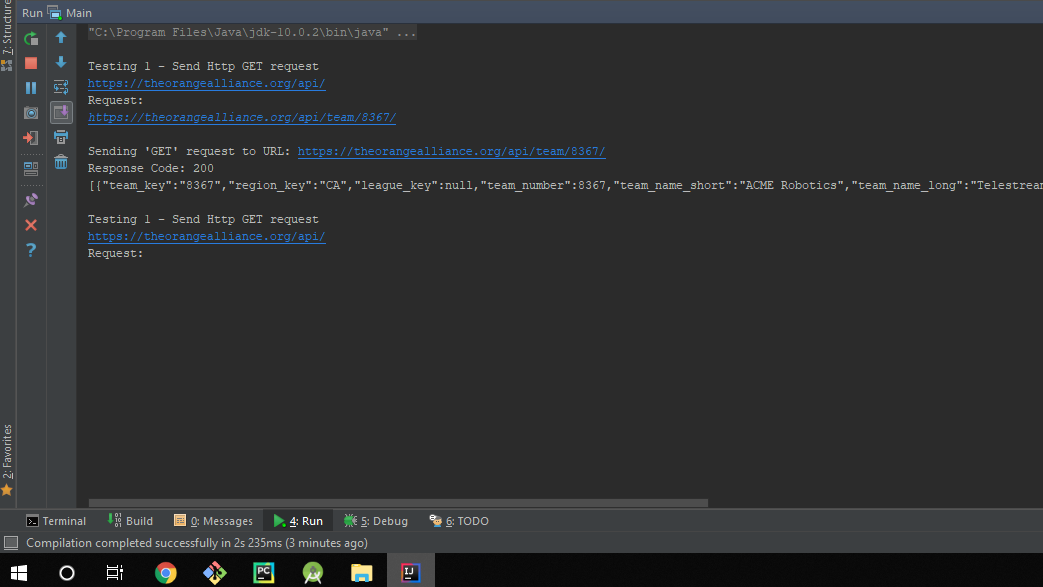
\includegraphics[width=.6 \textwidth]{15_12-10/images/console.png}
    \caption{The Console for the Prescouter}
    \label{fig:console}
\end{figure}

\end{document} 